%!TEX program = xelatex
% 完整编译: xelatex(cn) -> bibtex(cn) -> xelatex(cn) -> xelatex(cn) -> xelatex(en)
\documentclass[lang=en,11pt,a4paper,cite=numbers]{elegantpaper}
\usepackage{xfp}
\usepackage{tikz}

\title{Manifold}
\author{Hui Zheng}
% \institute{}

% \version{0.09}
\date{\today}

% 本文档命令
\usepackage{array}
\newcommand{\ccr}[1]{\makecell{{\color{#1}\rule{1cm}{1cm}}}}

\begin{document}

\maketitle

\begin{abstract}
  The definition of Manifold.
\keywords{Manifold}
\end{abstract}

\section{Manifold\cite{manifold}}
  A manifold is a topological space\ref{terms:topological-space} that is locally Euclidean (i.e., around every point, there is a neighborhood that is topologically the same as the open\ref{terms:open-set} unit ball in $\mathbb{R}^{n}$). To illustrate this idea, consider the ancient belief that the Earth was flat as contrasted with the modern evidence that it is round. The discrepancy arises essentially from the fact that on the small scales that we see, the Earth does indeed look flat. In general, any object that is nearly "flat" on small scales is a manifold, and so manifolds constitute a generalization of objects we could live on in which we would encounter the round/flat Earth problem, as first codified by Poincar$\rm{\acute{e}}$.

  More concisely, any object that can be "charted" is a manifold.
\begin{figure}[!htb]
  \centering
  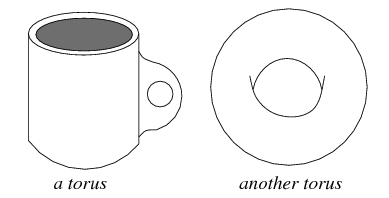
\includegraphics[width=0.4\textwidth]{figs/manifold.png}
  \caption{figs:manifold}
  \label{figs:manifold}
\end{figure}

  One of the goals of topology is to find ways of distinguishing manifolds. For instance, a circle is topologically the same as any closed loop, no matter how different these two manifolds may appear. Similarly, the surface of a coffee mug with a handle is topologically the same as the surface of the donut, and this type of surface is called a (one-handled) torus\ref{terms:torus}.

  As a topological space, a manifold can be compact or noncompact, and connected or disconnected. Commonly, the unqualified term "manifold"is used to mean "manifold with boundary." This is the usage followed in this work. However, an author will sometimes be more precise and use the term open manifold for a noncompact manifold without boundary or closed manifold for a compact manifold with boundary.

  If a manifold contains its own boundary, it is called, not surprisingly, a "manifold with boundary." The closed unit ball in $\mathbb{R}^n$ is a manifold with boundary, and its boundary is the unit sphere. The concept can be generalized to manifolds with corners. By definition, every point on a manifold has a neighborhood together with a homeomorphism of that neighborhood with an open ball in $\mathbb{R}^n$. In addition, a manifold must have a second countable topology. Unless otherwise indicated, a manifold is assumed to have finite dimension $n$, for $n$ a positive integer.

  Smooth manifolds (also called differentiable manifolds) are manifolds for which overlapping charts "relate smoothly" to each other, meaning that the inverse of one followed by the other is an infinitely differentiable map from Euclidean space to itself. Manifolds arise naturally in a variety of mathematical and physical applications as "global objects." For example, in order to precisely describe all the configurations of a robot arm or all the possible positions and momenta of a rocket, an object is needed to store all of these parameters. The objects that crop up are manifolds. From the geometric perspective, manifolds represent the profound idea having to do with global versus local properties.

  The basic example of a manifold is Euclidean space, and many of its properties carry over to manifolds. In addition, any smooth boundary of a subset of Euclidean space, like the circle or the sphere, is a manifold. Manifolds are therefore of interest in the study of geometry, topology, and analysis.

  A submanifold is a subset of a manifold that is itself a manifold, but has smaller dimension. For example, the equator of a sphere is a submanifold. Many common examples of manifolds are submanifolds of Euclidean space. In fact, Whitney showed in the 1930s that any manifold can be embedded in $\mathbb{R}^N$, where $N=2n+1$.

  A manifold may be endowed with more structure than a locally Euclidean topology. For example, it could be smooth, complex, or even algebraic (in order of specificity). A smooth manifold with a metric is called a Riemannian manifold, and one with a symplectic structure is called a symplectic manifold. Finally, a complex manifold with a Kähler structure is called a Kähler manifold.

\section{Topological Space\cite{topological-space}}
\label{terms:topological-space}
  A topological space, also called an abstract topological space, is a set $X$ together with a collection of open subsets $T$ that satisfies the four conditions:
\begin{enumerate}
  \item The empty set $\emptyset$ is in $T$.
  \item $X$ is in $T$.
  \item The intersection of a finite number of sets in $T$ is also in $T$.
  \item The union of an arbitrary number of sets in $T$ is also in $T$.
\end{enumerate}
Alternatively, $T$ may be defined to be the closed sets rather than the open sets, in which case conditions 3 and 4 become:
\newcounter{counter}
\setcounter{counter}{2}
\begin{enumerate}[\thecounter.]
  \stepcounter{counter}
  \item The intersection of an arbitrary number of sets in $T$ is also in $T$.
  \stepcounter{counter}
  \item The union of a finite number of sets in $T$ is also in $T$.
\end{enumerate}
These axioms are designed so that the traditional definitions of open and closed intervals of the real line continue to be true. For example, the restriction in (3) can be seen to be necessary by considering  $\cap_{(n=1)}^{\infty}(-\frac{1}{n},\frac{1}{n})=\{0\}$, where an infinite intersection of open intervals is a closed set.

  In the chapter "Point Sets in General Spaces" Hausdorff (1914) defined his concept of a topological space based on the four Hausdorff axioms (which in modern times are not considered necessary in the definition of a topological space).

\section{Open Set\cite{open-set}}
\label{terms:open-set}
\begin{figure}[!htb]
  \centering
  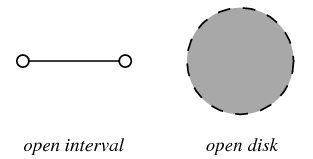
\includegraphics[width=0.4\textwidth]{figs/open-set.png}
  \caption{figs:open-set}
  \label{figs:open-set}
\end{figure}
  Let $S$ be a subset of a metric space. Then the set $S$ is open if every point in $S$ has a neighborhood lying in the set. An open set of radius $r$ and center $\textbf{x}_{0}$ is the set of all points $\textbf{x}$ such that $\left|\textbf{x}-\textbf{x}_{0}\right|{\le}r$, and is denoted $D_{r}(\textbf{x}_{0})$. In one-space, the open set is an open interval. In two-space, the open set is a disk. In three-space, the open set is a ball.

  More generally, given a topology(consisting of a set $X$ and a collection of subsets $T$), a set is said to open if it is in $T$. Therefore, while it is not possible for a set to be both finite and open in the topology of the real line(a single point is a closed set), it is possible for a more general topological set to be both finite and open.

  The complement of an open set is closed set. It is possible for a set to be neither open nor closed, e.g., the half-closed interval$(0,1]$.

\section{Torus\cite{torus}}
\label{terms:torus}
\begin{figure}[!htb]
  \centering
  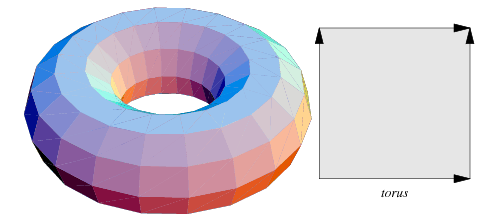
\includegraphics[width=0.6\textwidth]{figs/torus.png}
  \caption{figs:torus}
  \label{figs:torus}
\end{figure}
  An (ordinary) torus is a surface having genus\ref{terms:torus-genus} one, and therefore possessing a single "hole" (left figure). The single-holed "ring" torus is known in older literature as an "anchor ring." It can be constructed from a rectangle by gluing both pairs of opposite edges together with no twists (right figure; Gardner 1971, pp. 15-17; Gray 1997, pp. 323-324). The usual torus embedded in three-dimensional space is shaped like a donut, but the concept of the torus is extremely useful in higher dimensional space as well.

  In general, tori can also have multiple holes, with the term n-torus used for a torus with $n$ holes. The special case of a 2-torus is sometimes called the double torus, the 3-torus is called the triple torus, and the usual single-holed torus is then simple called "the" or "a" torus.

  A second definition for $n$-tori relates to dimensionality. In one dimension, a line bends into circle, giving the 1-torus. In two dimensions, a rectangle wraps to a usual torus, also called the 2-torus. In three dimensions, the cube wraps to form a 3-manifold, or 3-torus. In each case, the $n$-torus is an object that exists in dimension $n+1$. One of the more common uses of $n$-dimensional tori is in dynamical systems\ref{terms:torus-dynamical-systems}. A fundamental result states that the phase space trajectories of a Hamiltonian system with $n$ degrees of freedom and possessing $n$ integrals of motion lie on an $n$-dimensional manifold which is topologically equivalent to an $n$-torus (Tabor 1989).

  Torus coloring of an ordinary (one-holed) torus requires 7 colors, consistent with the Heawood conjecture.

  Let the radius from the center of the hole to the center of the torus tube be $c$, and the radius of the tube be $a$. Then the equation in Cartesian coordinates for a torus azimuthally symmetric about the z-axis is
\begin{equation}
   \left(c-\sqrt{(x^{2}+y^{2})}\right)^{2}+z^{2}=a^{2} 
\end{equation}
and the parametric equations are
\begin{equation}
  \begin{aligned}
    x&=(c+a\rm{cos}v)\rm{cos}u\\
    y&=(c+a\rm{cos}v)\rm{sin}u\\
    z&=a\rm{sin}v
  \end{aligned}
\end{equation}
for $u,v \in [0,2pi)$. Three types of torus, known as the standard tori, are possible, depending on the relative sizes of $a$ and $c$. $c>a$ corresponds to the ring torus (shown above), $c=a$ corresponds to a horn torus which is tangent to itself at the point (0, 0, 0), and $c<a$ corresponds to a self-intersecting spindle torus (Pinkall 1986).

  If no specification is made, "torus" is taken to mean ring torus. The three standard tori are illustrated below, where the first image shows the full torus, the second a cut-away of the bottom half, and the third a cross section of a plane passing through the z-axis.
\begin{figure}[!htb]
  \centering
  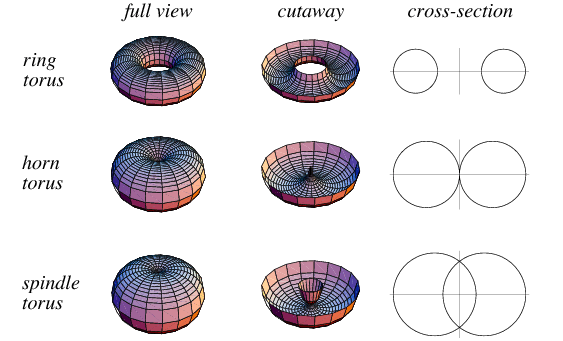
\includegraphics[width=0.6\textwidth]{figs/torus-types.png}
  \caption{figs:torus-types}
  \label{figs:torus-types}
\end{figure}

  The standard tori and their inversions are cyclides. If the coefficient of $\rm{sin}v$ in the formula for $z$ is changed to $b{\neq}a$, an elliptic torus results.
\begin{figure}[!htb]
  \centering
  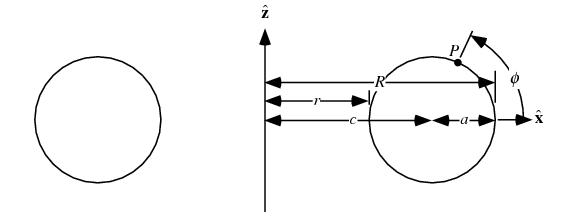
\includegraphics[width=0.6\textwidth]{figs/elliptic-torus.png}
  \caption{figs:elliptic-torus}
  \label{figs:elliptic-torus}
\end{figure}
To compute the metric properties of the ring torus, define the inner and outer radii by
\begin{equation}
  \begin{aligned}
    r&{\equiv}c-a\\
    R&{\equiv}c+a
  \end{aligned}
\end{equation}
Solving for a and c gives
\begin{equation}
  \begin{aligned}
    a&=\frac{1}{2}(R-r)\\
    c&=\frac{1}{2}(R+r)
  \end{aligned}
\end{equation}
Then the surface area of this torus is
\begin{equation}
  \begin{aligned}
    S&=(2{\pi}a)(2{\pi}c)\\
     &=4{\pi}^{2}ac\\
     &={\pi}^{2}(R+r)(R-r)^{2}
  \end{aligned}
\end{equation}
The volume can also be found by integrating the Jacobian computed from the parametric equations of the solid,
\begin{equation}
  \begin{aligned}
    x&=(c+r'\rm{cos}v)\rm{cos}u\\
    y&=(c+r'\rm{cos}v)\rm{sin}u\\
    z&=r'\rm{sin}v
  \end{aligned}
\end{equation}
which simplifies to
\begin{equation}
  \begin{aligned}
    J&=\left|\frac{{\partial}(x,y,z)}{{\partial}(u,v,r')}\right|=r'(c+r'\rm{cos}v)
  \end{aligned}
\end{equation}
giving
\begin{equation}
  \begin{aligned}
    V&=\int^{2\pi}_{0}\int^{2\pi}_{0}\int^{a}_{0}r'(c+r'\rm{cos}v)dr'dudv\\
     &=2{\pi}^{2}a^{2}c
  \end{aligned}
\end{equation}
as before.

  The moment of inertia tensor of a solid torus with mass $M$ is given by
\begin{equation}
  \begin{aligned}
    V&=\begin{bmatrix}
      (\frac{5}{8}a^{2}+\frac{1}{2}c^{2})M & 0 & 0 \\
      0 & (\frac{5}{8}a^{2}+\frac{1}{2}c^{2})M & 0 \\
      0 & 0 & (\frac{3}{4}a^{2}+c^{2})M
    \end{bmatrix}
  \end{aligned}
\end{equation}
The coefficients of the first fundamental form are
\begin{equation}
  \begin{aligned}
    E&=(c+a\rm{cos}v)^{2}\\
    F&=0\\
    G&=a^{2}
  \end{aligned}
\end{equation}
and the coefficients of the second fundamental form are
\begin{equation}
  \begin{aligned}
    e&=-(c+a\rm{cos}v)\rm{cos}v\\
    f&=0\\
    G&=-a
  \end{aligned}
\end{equation}
giving Riemannian metric
\begin{equation}
  \begin{aligned}
    ds^{2}&=(c+a\rm{cos}v)^{2}du^{2}+a^{2}dv^{2}
  \end{aligned}
\end{equation}
area element
\begin{equation}
  \begin{aligned}
    dA&=a(c+a\rm{cos}v)du{\land}dv
  \end{aligned}
\end{equation}
(where $du{\land}dv$ is a wedge product), and Gaussian and mean curvatures as
\begin{equation}
  \begin{aligned}
    K&=\frac{\rm{cos}v}{a(c+a\rm{cos}v)}\\
    H&=-\frac{c+2a\rm{cos}v}{2a(c+a\rm{cos}v)}
  \end{aligned}
\end{equation}
(Gray 1997, pp. 384-386).

  A torus with a hole in its surface can be turned inside out to yield an identical torus. A torus can be knotted externally or internally, but not both. These two cases are ambient isotopies, but not regular isotopies. There are therefore three possible ways of embedding a torus with zero or one knot.
\begin{figure}[!htb]
  \centering
  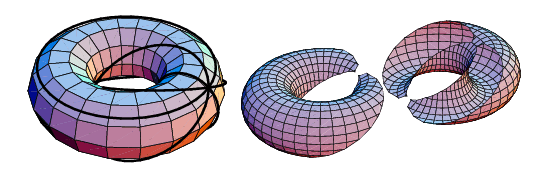
\includegraphics[width=0.6\textwidth]{figs/ambient-isotopies.png}
  \caption{figs:ambient-isotopies}
  \label{figs:ambient-isotopies}
\end{figure}

  An arbitrary point P on a torus (not lying in the xy-plane) can have four circles drawn through it. The first circle is in the plane of the torus and the second is perpendicular to it. The third and fourth circles are called Villarceau circles (Villarceau 1848, Schmidt 1950, Coxeter 1969, Melnick 1983).

\subsection{Genus\cite{genus}}
\label{terms:torus-genus}
  A topologically invariant property of a surface defined as the largest number of nonintersecting simple closed curves that can be drawn on the surface without separating it. Roughly speaking, it is the number of holes in a surface.

  The genus of a surface, also called the geometric genus, is related to the Euler characteristic\ref{terms:torus-euler-characteristic} $\chi$. For a orientable surface such as a sphere (genus 0) or torus (genus 1), the relationship is
\begin{equation}
  {\chi}=2-2g
\end{equation}

  For a nonorientable surface such as a real projective plane (genus 1) or Klein bottle (genus 2), the relationship is
\begin{equation}
  {\chi}=2-g
\end{equation}
(Massey 2003).

\subsection{Euler Characteristic\cite{euler-characteristic}}
\label{terms:torus-euler-characteristic}
  Let a closed surface have genus g. Then the polyhedral formula generalizes to the Poincar$\rm{\acute{e}}$ formula
\begin{equation}
  {\chi}(g){\equiv}V-E+F,
\end{equation}
where
\begin{equation}
  {\chi}(g)=2-2g
\end{equation}
is the Euler characteristic, sometimes also known as the Euler-Poincar$\rm{\acute{e}}$ characteristic. The polyhedral formula corresponds to the special case $g=0$.

  The only compact closed surfaces with Euler characteristic 0 are the Klein bottle and torus (Dodson and Parker 1997, p. 125). The following table gives the Euler characteristics for some common surfaces (Henle 1994, pp. 167 and 295; Alexandroff 1998, p. 99).
\begin{table}[htbp]
  \centering
  \begin{tabular}{c|c}
    \hline
    surface & $\chi$ \\
    \hline
    cylinder & 0 \\
    double torus & -2 \\
    Klein bottle & 0 \\
    M$\rm{\ddot{o}}$bius strip & 0 \\
    projective plane & 1 \\
    sphere & 2 \\
    torus & 0 \\
    \hline
  \end{tabular}
\end{table}

  In terms of the integral curvature of the surface $K$,
\begin{equation}
  {\iint}Kda=2{\pi}{\chi}
\end{equation}
The Euler characteristic is sometimes also called the Euler number. It can also be expressed as
\begin{equation}
  {\chi}=p_{0}-p_{1}+p_{2}
\end{equation}
where $p_i$ is the ith Betti number of the space.

\subsection{Dynamical Systems\cite{dynamical-systems}}
\label{terms:torus-dynamical-systems}
  A means of describing how one state develops into another state over the course of time. Technically, a dynamical system is a smooth action of the reals or the integers on another object (usually a manifold). When the reals are acting, the system is called a continuous dynamical system, and when the integers are acting, the system is called a discrete dynamical system. If $f$ is any continuous function, then the evolution of a variable $x$ can be given by the formula
\begin{equation}
  x_{n+1}=f(x_{n})
\end{equation}
This equation can also be viewed as a difference equation
\begin{equation}
  x_{n+1}-x_{n}=f(x_{n})-x_{n}
\end{equation}
so defining
\begin{equation}
  g(x){\equiv}f(x)-x
\end{equation}
gives
\begin{equation}
  x_{n+1}-x_{n}=g(x_{n})*1
\end{equation}
which can be read "as $n$ changes by 1 unit, $x$ changes by $g(x)$." This is the discrete analog of the differential equation
\begin{equation}
  x'(n)=g(x(n))
\end{equation}

%\nocite{*}
\bibliography{ref/refs}

\end{document}
